\documentclass[11pt,a4paper]{article}
\usepackage[utf8]{inputenc}
\usepackage[spanish]{babel}
\usepackage[margin=2.5cm]{geometry}
\usepackage{graphicx}
\usepackage{amsmath,amssymb}
\usepackage{booktabs}
\usepackage{longtable}
\usepackage{array}
\usepackage{hyperref}
\usepackage{listings}
\usepackage{xcolor}
\usepackage{caption}
\usepackage{float}

\graphicspath{{figuras/}}

\lstset{
  basicstyle=\ttfamily\footnotesize,
  breaklines=true,
  columns=fullflexible,
  backgroundcolor=\color{gray!8},
  frame=single,
  language=Matlab,
  commentstyle=\color{gray},
  keywordstyle=\color{blue!60!black}
}

\hypersetup{colorlinks=true, linkcolor=blue!40!black, citecolor=blue!40!black, urlcolor=blue!40!black}

\title{Control continuo mioeléctrico con TD3 y permiso de movimiento externo:\\
del guante físico a \texttt{motionPermission}\\
\large Historia completa del experimento \emph{no-glove-intent-control}, ETAPA 0 a ETAPA 7U}
\author{Proyecto EMG\_Prosthesis\_TD3 --- Laboratorio de Inteligencia y Visión Artificial\\
Escuela Politécnica Nacional, Quito, Ecuador}
\date{Compilado el \today}

\begin{document}
\maketitle
\tableofcontents
\newpage

\section{Introducción y objetivo}

Este documento consolida la investigación completa del proyecto de control continuo y
proporcional de una prótesis mioeléctrica de cuatro motores, desde la arquitectura
histórica basada en un guante instrumentado hasta la línea experimental actual,
que elimina el guante y controla la prótesis exclusivamente a partir de electromiografía
(EMG) de superficie, usando un actor TD3 (\emph{Twin Delayed DDPG}) cuya salida cruda
se combina con una compuerta causal externa de permiso de movimiento
(\texttt{motionPermission}) antes de llegar a la capa determinista de seguridad y a la
cuantización PWM.

El objetivo declarado del proyecto \textbf{no} es clasificar únicamente gestos
discretos, sino lograr control continuo manteniendo: seguimiento (\emph{tracking})
adecuado de la referencia, acciones suaves, baja saturación, seguridad mecánica,
comportamiento coherente durante el reposo y ausencia de movimiento no solicitado.

Todo el contenido cuantitativo de este informe proviene de artefactos realmente
ejecutados y guardados en disco (checkpoints, logs por episodio, \texttt{training\_info},
tablas CSV) --- no de proyecciones ni de extrapolaciones. Cuando una cifra corresponde a
una corrida específica se cita su carpeta de salida.

\section{Arquitectura histórica con guante}

\subsection{Agent7250 y el benchmark histórico}

La línea original del proyecto (ETAPA 0, previa a este experimento) usaba un guante
instrumentado como fuente de referencia de posición, junto con un controlador
entrenado por refuerzo (\texttt{Agent7250\_valid\_baseline}) que sirve como benchmark
histórico congelado. La auditoría de línea base (\texttt{00\_baseline\_audit.md})
encontró y documentó:

\begin{itemize}
  \item métricas canónicas congeladas: \texttt{trackingMSE}=0.043045,
    \texttt{MAE}=0.160336, \texttt{actionL2}=0.596444,
    \texttt{saturationFraction}=0.392086, \texttt{deltaActionL2}=0.321385;
  \item acoplamiento estructural profundo al guante en el constructor, \texttt{reset},
    \texttt{step}, reward y condición de terminación de \texttt{Env};
  \item que \texttt{simMotors=true} \textbf{no} bloqueaba por sí solo una conexión real
    al brazalete Myo --- hallazgo que resultó central más adelante, al preparar la
    fase Myo (Sección~\ref{sec:myo});
  \item que las propiedades \texttt{Constant} de la clase \texttt{Env} podían ocultar
    sobrescrituras de configuración entre corridas.
\end{itemize}

\subsection{Problemas originales y saturación histórica}

El benchmark histórico mostraba saturación de acción alta (\texttt{saturationFraction}
$\approx 0.39$) y una fuerte dependencia del guante como única fuente de referencia
mecánicamente viable. Esto motivó la línea experimental \emph{no-glove}: sustituir el
guante por un decodificador de intención basado exclusivamente en EMG cruda, generando
una referencia de posición/velocidad mecánicamente acotada sin necesidad de un sensor
de posición externo.

\section{Eliminación del guante: arquitectura EMG-only}

La arquitectura conceptual completa de la línea \emph{no-glove} es:

\begin{center}
EMG cruda $\to$ calibración de sesión $\to$ extracción de features $\to$
decoder de intención $\to$ referencia mecánicamente viable
$\to$ estado causal del controlador $\to$ actor TD3 $\to$ acción cruda
$\to$ \texttt{motionPermission} $\to$ acción solicitada
$\to$ capa determinista de seguridad $\to$ cuantización/PWM $\to$ simulador/planta.
\end{center}

\subsection{Calibración de sesión}

\texttt{calibrateEmgIntent.m} calibra, a partir de una captura de reposo y de ensayos
de instrucción por canal, un decodificador lineal de rango~2 (\texttt{r=2}) mediante
regresión ridge sobre \texttt{atanh} de la actividad normalizada. La calibración
resultante incluye, entre otros campos: \texttt{baselineMedian}, \texttt{signalLevel},
\texttt{activeChannelMask}, la matriz de decodificador \texttt{decoder.W}/\texttt{bias},
la matriz de sinergia motor (\texttt{synergy.matrix}), los límites mecánicos
(\texttt{limits.positionMin/Max/velocityMax/accelerationMax/deltaT}) y los umbrales de
histéresis del gate de reposo (\texttt{restGate.thetaOn/thetaOff/nOn/nOff}). Un checksum
SHA-256 (\texttt{computeIntentCalibrationChecksum.m}) protege el contrato completo contra
mezclas accidentales entre sesiones/usuarios.

\subsection{Envelope y features}

\texttt{computeEmgEnvelope.m} calcula la envolvente de valor absoluto medio por ventana
no solapada (\texttt{windowLengthSamples}/\texttt{hopLengthSamples}), previa e
independiente de cualquier estandarización WMoos. Para el estado del controlador,
\texttt{getWmoosFeatures} produce 40 features EMG normalizadas por canal con las
constantes \texttt{C}/\texttt{S} de \texttt{normValues.mat} --- un archivo histórico de
39\,MB cuya procedencia exacta \emph{no} está documentada con metadatos de
sesión/usuario/orden de canal (hallazgo de auditoría, ver Sección~\ref{sec:auditoria-pipeline}).

\subsection{Decoder de intención}

\texttt{mapEmgToIntentVelocity.m} decodifica cada ventana EMG cruda causal en una
velocidad de intención de 4 motores, mediante:

\begin{enumerate}
  \item normalización de la envolvente contra la línea base de reposo
    (\texttt{baselineMedian}/\texttt{signalLevel});
  \item un gate de histéresis de dos umbrales sobre la actividad promedio de los
    canales activos: entra en actividad tras \texttt{nOn} ventanas consecutivas por
    encima de \texttt{thetaOn}, y vuelve a reposo tras \texttt{nOff} ventanas
    consecutivas por debajo de \texttt{thetaOff} (\texttt{thetaOn>thetaOff}, evita
    \emph{chattering});
  \item durante la cuenta regresiva de baja actividad previa al cierre del gate
    (\texttt{lowActivityCountdown}), la velocidad de intención se fuerza a cero --- un
    frenado acotado antes de declarar reposo exacto;
  \item sólo cuando el gate está activo y fuera de esa cuenta regresiva, la intención
    decodificada (\texttt{tanh} de la proyección lineal) se transforma en velocidad de
    motor vía la matriz de sinergia y \texttt{velocityMax}.
\end{enumerate}

\subsection{Referencia mecánicamente viable: \texorpdfstring{$q_{ref}$}{q\_ref}/\texorpdfstring{$v_{ref}$}{v\_ref}}

\texttt{updateIntentReference.m} integra la velocidad decodificada respetando límites
de posición, velocidad y aceleración, y --- crucialmente --- congela exactamente la
referencia (\texttt{q\_ref} constante, \texttt{v\_ref=0}) cuando el gate declara reposo
(\texttt{restMask}). Esta es la primera y más fundamental garantía de seguridad de la
arquitectura: \emph{la referencia nunca pide movimiento durante el reposo declarado},
independientemente de lo que haga después el actor TD3.

\subsection{\texttt{intentMarkov60}}

El estado observado por el actor (ETAPA 3) concatena, en este orden exacto
(\texttt{buildObservationLayout.m}):

\begin{center}
\begin{tabular}{lll}
\toprule
Bloque & Dimensiones & Contenido \\
\midrule
EMG & 1--40 & 40 features WMoos normalizadas \\
encoder & 41--44 & posición normalizada $q$ \\
deltaEncoder & 45--48 & $\Delta q = q_t - q_{t-1}$ (acotado a $[-1,1]$) \\
previousEffectiveAction & 49--52 & acción efectiva aplicada en $t-1$ \\
referencePosition & 53--56 & $q_{ref,t}$ \\
referenceVelocity & 57--60 & $v_{ref,t}$ \\
\bottomrule
\end{tabular}
\end{center}

Toda la cadena de actualización es estrictamente causal: la EMG leída durante la
transición $t$ actualiza el decodificador y la referencia \emph{después} de que el
reward de la acción $a_t$ ya fue evaluado contra lo visible en el estado $t$, y sólo
entonces se construye el estado $t+1$ (\texttt{advanceIntentReference.m},
\texttt{Env/step.m}).

\subsection{Experimento \texttt{intentMarkov62}: \texttt{declaredRest}/\texttt{holdLatch}}

ETAPA 7M extendió el estado a 62 dimensiones añadiendo dos bits observables:
\texttt{declaredRest} (reposo declarado por el gate) y \texttt{holdLatch} (memoria
causal de mantenimiento de posición, ver \texttt{updateIntentDeclaredRestHoldState.m}).
La integración fue validada con regresión exacta cero frente a las primeras 60
dimensiones. Sin embargo, ETAPA 7N (entrenamiento con \texttt{intentMarkov62}) y
ETAPA 7O (contrafactual de esos bits sobre el actor congelado) mostraron que
\textbf{exponer la información no basta}: el actor de 62 entradas es sensible a los
bits, pero el efecto es dependiente de contexto y motor, sin combinación universal que
lo convierta en un inhibidor robusto de reposo. La recomendación de 7O fue volver a
\texttt{intentMarkov60} para entrenamiento y \emph{no} seguir añadiendo bits al estado
sin una hipótesis nueva --- precondición directa de la arquitectura híbrida final
(Sección~\ref{sec:motion-permission}).

\section{Reward}

La línea causal de intención usa \texttt{trackingIntentActionRateReward.m}:

\begin{align}
r_t = -\frac{1}{4}\sum_{i=1}^{4} \Big[
  & w_Q\,(q_{i} - q_{ref,i})^2
  + w_V\,(\dot q_i - v_{ref,i})^2 \nonumber\\
  & + w_U\, u_{eff,i}^2
  + w_{\Delta U}\,(u_{eff,i} - u_{eff,i}^{t-1})^2 \nonumber\\
  & + w_{sat}\,\max(0, |u_{eff,i}| - u_{soft})^2
  \Big]
\end{align}

con pesos vigentes (\texttt{configurables.m}): $w_Q=1.00$, $w_V=0.00$, $w_U=0.01$,
$w_{\Delta U}=0.05$, $w_{sat}=0.02$, $u_{soft}=0.90$.

\textbf{Cada término, explicado:}
\begin{itemize}
  \item $w_Q$ (posición): penaliza el error de seguimiento; domina el reward por dos
    órdenes de magnitud sobre $w_U$.
  \item $w_V$ (velocidad): actualmente inerte (peso cero) en el perfil vigente ---
    el error de velocidad se diagnostica en \texttt{rewardInfo} pero no se incentiva.
  \item $w_U$ (esfuerzo): penaliza la magnitud de la acción \emph{efectiva}
    (post-gate, post-cuantización), \textbf{no} la acción cruda del actor.
  \item $w_{\Delta U}$ (suavidad): penaliza el cambio de acción efectiva entre pasos
    consecutivos; su peso es 5$\times$ mayor que $w_U$, lo que castiga más
    \emph{cambiar} de acción que \emph{mantenerla}.
  \item $w_{sat}$ (saturación blanda): penaliza cuadráticamente el exceso sobre
    $u_{soft}=0.90$, antes de la saturación dura en $\pm1$.
\end{itemize}

\textbf{Hallazgo de auditoría (Sección~\ref{sec:auditoria-pipeline}):} como el reward
usa la acción \emph{efectiva} y no la cruda, durante los pasos con
\texttt{motionPermission} inactivo el reward es \emph{idéntico} sin importar la
magnitud de $u_{actor,raw}$ --- el crítico no recibe gradiente que discipline al actor
en esos pasos. Esto es una consecuencia correcta y deseada del diseño, no un error: ya
no se le exige al actor aprender a no moverse en reposo, porque el permiso externo lo
garantiza estructuralmente.

\section{Cuantización, PWM y seguridad}

\texttt{remapActionForActuator.m} cuantiza la acción (ya gateada) a niveles PWM
discretos $\{0,64,96,128,160,192,224,255\}$ con umbral de activación
\texttt{actionCommandActivationThreshold=0.05}. La capa de seguridad
(\texttt{limitSimulationPosition.m}), quirúrgicamente externa al simulador de planta,
recorta la trayectoria simulada a los límites de posición calibrados
(\texttt{simulationPositionSafety.positionMin/Max}), y conserva siempre autoridad
final --- \texttt{motionPermission} actúa \emph{antes} de esta capa, nunca la
reemplaza ni se aplica después de ella.

\section{Simulador}

\texttt{prosthesis\_simulator.m} no integra una física paramétrica: reproduce curvas de
trayectoria ajustadas empíricamente por motor y velocidad (\texttt{fit\_C2.mat},
\texttt{pattern\_curve.mat}), indexadas por duración transcurrida. Un hallazgo de
auditoría de ETAPA~7T (Sección~\ref{sec:etapa7t}) mostró que el índice de esa curva se
satura en su longitud grabada: sostener PWM máximo indefinidamente no mueve la posición
más allá de ese punto --- un equilibrio genuino del simulador, no necesariamente igual
al límite calibrado idealizado \texttt{positionMax=1}.

\section{El problema de reposo: etapas 7A a 7T}

La Tabla~\ref{tab:etapas} resume, etapa por etapa, la investigación completa desde la
línea base histórica (ETAPA 0) hasta el cierre de ETAPA 7T. Cada fila refleja
\emph{exactamente} lo que el documento de la etapa correspondiente declara --- no se
infieren resultados no documentados.

\begin{longtable}{p{1.3cm}p{3.1cm}p{3.3cm}p{3.6cm}p{1.6cm}p{3.4cm}}
\caption{Historial completo de etapas, ETAPA 0 a ETAPA 7T.}
\label{tab:etapas}\\
\toprule
Etapa & Hipótesis & Cambio & Métricas/Evidencia & Result. & Conclusión \\
\midrule
\endfirsthead
\toprule
Etapa & Hipótesis & Cambio & Métricas/Evidencia & Result. & Conclusión \\
\midrule
\endhead
00 & Orientar el repo, congelar benchmark histórico & Sin cambios de código; se congeló Agent7250 & trackingMSE=0.043, satFrac=0.392 & PASS & Fuerte acoplamiento al guante; decoplar en Etapa 1 \\
01 & ¿Se puede desacoplar la fuente de referencia sin alterar el guante? & \texttt{referenceSource} de instancia; \texttt{emgIntent} salta carga de guante & 0 discrepancias en regresión de 50 episodios & PASS & Desacoplamiento logrado sin regresión \\
02 & ¿Es correcta la cadena envolvente$\to$calibración$\to$decoder$\to$histéresis? & \texttt{computeEmgEnvelope}, \texttt{calibrateEmgIntent}, histéresis & RMSE=0.0082, 0 falsas activaciones & PASS (fixture sintético) & No demuestra separabilidad humana real \\
03 & ¿\texttt{intentMarkov60} se integra causalmente sin regresión? & \texttt{buildObservationLayout}, \texttt{advanceIntentReference} & Residuales de alineación causal = 0 exacto & PASS & Estado causal íntegro; $a_t$ nunca ve info de $t+1$ \\
04 & ¿Reward causal correcto sin DTW? & \texttt{trackingIntentActionRateReward} & Residual máx. $5.55\times10^{-17}$ & PASS & Validado numéricamente \\
05 & Caracterizar planta P/PD sin tocar el simulador & Diagnóstico offline & Inversión de signo en M2 & PASS (diag.) & Planta no corregida aún \\
06 & TD3 desde cero, ¿pasa el gate de 200 episodios? & Nuevo agente feedforward de 60 entradas & Posición 200/200 fuera; funcional FAIL & PARTIAL & Seguridad de posición pendiente \\
06A & ¿Clip determinista soluciona la posición? & \texttt{limitSimulationPosition} & 0 violaciones de posición; funcional persiste & PARTIAL & Seguridad $\neq$ control funcional \\
06B & ¿Qué explica la inmovilidad/actividad de reposo? & Analizador offline & 87.5\% inmovilidad; 44\% PWM$\neq$0 interior & PASS (diag.) & Sin causa única \\
06C & ¿El propio TD3 explica el esfuerzo/reposo? & Controlador P emparejado & P: 0 acción en reposo vs 876 intervenciones Agent200 & PASS (diag.) & Agent200 explica gran parte, no todo \\
07 & ¿El desfase temporal explica el error? & Barrido de lag + DTW restringido & Beneficio $<5\%$ & PASS ing.; DTW NO aprobado & Etapa 8 no autorizada \\
07A & ¿Óptimos de lag reproducibles? & LORO 6-fold & Óptimo en frontera 100\% de folds & NO aprobado & \texttt{temporalPatternUnresolved} \\
07B & Excitación diseñada, ¿lag genuino? & 16 perfiles sintéticos & Comandos antes de activarse la referencia & NO aprobado & Actividad anticipatoria, no lag \\
07C & ¿Qué en el estado causa PWM en reposo? & Réplica de actor congelado & 128/128 ventanas de reposo con PWM$\neq$0 & PASS ing. & Bloque EMG identificable, no aislable \\
07D & ¿Reposo fuera de soporte de entrenamiento? & Test de soporte MAD & Soporte EMG 0\%; reposo real también comanda & PASS ing. & \texttt{trainingRestAlsoCommands} \\
07E & ¿Desde cuándo aparece? & Réplica Agent50/100/150/200 & Fracción de comando = 1.0 desde Agent50 & PASS ing. & Presente desde el primer checkpoint \\
07F & ¿Subir $w_U$ lo resuelve? & Ablación pareada $w_U{=}0.05$ & PWM reposo 100\% en ambos & FAIL científico & Hipótesis rechazada \\
07G & ¿Umbral único separa reposo/movimiento? & Barrido offline de umbral & Pérdida de movimiento $>79\%$ & FAIL & No separable por umbral \\
07H & ¿Penalización de \emph{hold} en el reward? & \texttt{trackingIntentHoldActionReward} & Cobertura 53\%; MSE $8\times$ peor & FAIL & Cobertura insuficiente \\
07I & ¿Otro $\epsilon$ de posición? & Barrido offline & Ningún $\epsilon$ da 90\% cobertura + $\leq$5\% riesgo & FAIL & No separable \\
07J & ¿Latch geométrico causal? & Máquina de estados offline & Exposición lejana 20.8\% & FAIL & \texttt{latchedHoldNotSeparableFromFarCorrection} \\
07K & ¿Qué explica $v_{ref}=0$? & Réplica de decoder/referencia & 78\% \texttt{decoderRest}, 19\% \texttt{activeCountdownZero} & PASS ing. & $v_{ref}=0 \neq$ reposo declarado \\
07L & ¿Latch semántico (no geométrico)? & Latch por procedencia & 100\% cobertura, 0 fugas & PASS (científico) & Propone $s_{62}$ \\
07M & Implementar $s_{62}$ sin regresión & Nueva variante 62-dim & Diff. máx. vs $s_{60}$ = 0 exacto & PASS & Implementado, sin entrenar aún \\
07N & ¿Entrenar con $s_{62}$ mejora? & TD3 60 vs 62 entradas & PWM reposo 100\% en ambos & FAIL científico & Observabilidad sola no basta \\
07O & ¿El actor usa los bits 61/62? & Contrafactual + gradientes & Sensible, sin combinación universal & PASS ing. & \texttt{bitsContextDependent}; volver a $s_{60}$ \\
07P & ¿Cuantizador o gate-motor inactivo? & Estratificación offline & Ambas hipótesis fallan su umbral & PASS ing. & \texttt{noAblationSupported} \\
07Q & ¿Un bloque de estado domina? & Gradiente/asociación & EMG domina pero no es único ($q$ casi colineal con $q_{ref}$) & PASS ing. & \texttt{distributedOrUnresolved} \\
07R & ¿Una familia de features EMG? & Pares reales emparejados & \texttt{crossEpisode} 0/4 motores & PASS ing. & \texttt{insufficientMatchedSupport} \\
07S & ¿Corpus prospectivo de estrés del gate? & 80 episodios sintéticos & PWM$\neq$0=0.98125, satFrac=0.209, 4072 intervenciones & PASS ing. & \texttt{prospectiveSupportFailed} (pares insuficientes) \\
07T & ¿PWM firstStep es no solicitado? & Estratificación \texttt{firstStep}/\texttt{postFirst} & 7/7 canales, 4/4 motores $\geq$50\% PWM$\neq$0 & PASS (tras corrección, ver \S\ref{sec:etapa7t}) & \texttt{broadSyntheticGateStressConsequence} \\
\bottomrule
\end{longtable}

\subsection{Corrección de ETAPA 7T}
\label{sec:etapa7t}

La primera corrida de ETAPA 7T resultó \texttt{auditInvalid}: el supuesto de que los 80
episodios \texttt{firstStep} comienzan en el límite mecánico calibrado
(\texttt{positionMax=1}) resultó falso para los 40 episodios de tipo \emph{Opening}, que
se estabilizan en un punto reproducible ($\sigma\approx2\times10^{-16}$ entre episodios)
muy por debajo de 1 --- el equilibrio genuino de la curva empírica del simulador
(Sección anterior), no un error de causalidad. Se corrigió \emph{únicamente} el script
de auditoría offline (\texttt{deriveNoGloveStage7tReachableEndpoints.m}), anclando el
invariante al equilibrio mecánico certificado en lugar de al límite idealizado, sin
tocar datos, simulador, seguridad ni reward. Tras la corrección, ETAPA 7T clasificó
como \texttt{broadSyntheticGateStressConsequence}: en el primer paso (referencia
congelada, sin acción previa, demanda de control exactamente cero), 7 de 7 canales
dominantes y 4 de 4 motores comandan PWM no solicitado en $\geq$50\% de sus componentes,
con intervenciones de seguridad ya presentes.

\section{\texttt{motionPermission}: arquitectura híbrida final}
\label{sec:motion-permission}

La recomendación directa de ETAPA 7T (\texttt{preregisterSingleFactorGateAggregationAblation})
motivó ETAPA 7U: separar \emph{permiso de movimiento} de \emph{magnitud de control
continuo}, reutilizando --- no inventando --- la señal de gate ya validada
causalmente en 7K/7L:

\begin{center}
$u_{actor,raw}$ (actor congelado) $\xrightarrow{\text{permission}=\text{gateActive}_t}$
$u_{requested} = \text{permission}\cdot u_{actor,raw}$
$\xrightarrow{\text{remapActionForActuator}}$ PWM
$\xrightarrow{\text{limitSimulationPosition}}$ planta.
\end{center}

Justificación estructural: \texttt{updateIntentReference.m} ya fuerza $v_{ref}=0$
exactamente cuando \texttt{gateActive=false}. Aplicar el mismo booleano al actor
\emph{no puede}, por construcción, suprimir un movimiento que la referencia esté
pidiendo: cuando la referencia pide movimiento, \texttt{gateActive=true} y la acción
solicitada es idéntica a la cruda.

\textbf{Validación offline (contrafactual exacto, sin recargar el actor):} sobre 80
episodios de estrés sintético de ETAPA 7S, \texttt{restPWMNonZeroFraction} cae de
0.9812 a \textbf{0} exacto; sobre 50 episodios reales históricos de aceptación de
Agent200, 0 de 3050 pasos de inhibición falsa.

\textbf{Confirmación en lazo cerrado real:} se recargó Agent200 y se re-ejecutó en vivo
(sin reentrenar) sobre el mismo corpus determinista, con y sin el gate:
\texttt{trackingMse} \textbf{mejora} de 0.0123 a 0.0097 ($-21\%$), \texttt{actionL2} de
0.2471 a 0.1220 ($-50.6\%$), PWM de reposo intra-episodio de 100\% a 0\%.

\section{Auditoría del pipeline de entrenamiento}
\label{sec:auditoria-pipeline}

Antes de cualquier campaña larga se auditó, en el código fuente real del toolbox de RL
de MATLAB (\texttt{+rl/+env/+internal/MATLABSimulator.m}, función \texttt{simInternal\_},
líneas $\approx$104--124), el recorrido completo:

\begin{lstlisting}
act = evaluateAction(expProcessor, obs);   % salida del actor (con ruido si entrena)
[nobs, rwd, isd] = step(this, act);        % this = Env; act se pasa SIN modificar
exp.Action = rl.util.cellify(act);         % exactamente u_actor_raw
exp.Reward = rwd;                          % refleja la ejecucion YA gateada
\end{lstlisting}

\textbf{Confirmado, no inferido:} \texttt{exp.Action} --- lo que aprende el crítico ---
es exactamente $u_{actor,raw}$, capturado \emph{antes} de \texttt{step()}. El gate,
que sólo modifica la variable local \texttt{warpedAction} dentro de \texttt{step.m},
es invisible para ese registro. \texttt{exp.Reward}/\texttt{exp.NextObservation} sí
reflejan la ejecución real (gateada). Esto es coherente: crítico y actor aprenden sobre
el mismo espacio de acción ($u_{raw}$), y la recompensa corresponde genuinamente a lo
que el entorno hizo con esa acción.

\textbf{Distinción \texorpdfstring{$u_{actor,raw}$}{u\_actor\_raw} vs
\texorpdfstring{$u_{requested}$}{u\_requested} vs
\texorpdfstring{$u_{effective}$}{u\_effective}:}
\begin{itemize}
  \item $u_{actor,raw}$ (\texttt{actionLog}): salida directa del actor, con ruido de
    exploración durante entrenamiento; \textbf{nunca} modificada por el gate.
  \item $u_{requested}$ (\texttt{actionWarpLog}): $u_{raw}$ tras aplicar
    \texttt{motionPermission} (cero si el permiso está inactivo) y el posible
    \emph{warp} de interfaz de acción.
  \item $u_{effective}$ (\texttt{actionSatLog}): $u_{requested}$ tras cuantización a
    niveles PWM discretos --- es lo que realmente ve el reward y la planta.
\end{itemize}

\textbf{Replay buffer y crítico:} el buffer de experiencia de \texttt{rlTD3Agent} usa
muestreo uniforme (sin \emph{prioritized replay}); para la línea auditada,
\texttt{agentNoGloveIntentTd3.m} fuerza \texttt{newTraining=true} y buffer reseteado ---
sin contaminación por \emph{warm-start} de corridas anteriores. \texttt{EpisodeQ0}
(estimación del crítico en el estado inicial de cada episodio) se recupera sin ningún
cambio de entrenamiento vía \texttt{trainingInfo.EpisodeQ0} (objeto
\texttt{rl.train.rlTrainingResult} devuelto por \texttt{train()}); las pérdidas de
actor/crítico por paso \textbf{no} están expuestas nativamente por \texttt{train()}
para TD3 (sólo para agentes MBPO) --- no se fuerza una extracción no soportada.

No se encontró ningún \emph{mismatch} acción/reward/replay. Se corrigieron dos brechas
reales (no de causalidad): \texttt{trainingInfo} se descartaba tras entrenar
(corregido, ahora se guarda con reward/pasos/Q0 por episodio), y un test determinista
nuevo (\texttt{testRewardUsesGatedActionNotRawAction}) confirma que el reward usa la
acción gateada, no la cruda.

\section{Piloto de 500 episodios}

Con \texttt{motionPermissionEnabled=true} desde el episodio 1 (actor nuevo, no
Agent200), 500 episodios: reward mejora de $-11.7$ a $-1.9$; \texttt{trackingMse} de
entrenamiento de 0.137 a 0.025; \texttt{restPwmNonZeroFraction}=0 exacto en las 100
muestras de entrenamiento guardadas y en las 50 evaluaciones finales, sin excepción. El
agente de 500 episodios \emph{aún no alcanza} a Agent200+\texttt{motionPermission}
(\texttt{trackingMse}=0.0137 vs 0.0097; \texttt{actionL2}=0.4342 vs 0.1220) --- esperado,
no una falla: con el gate activo desde el inicio, sólo $\approx$47.5\% de los pasos
aportan señal de aprendizaje efectiva.

\section{Campaña larga de 10\,000 episodios}
\label{sec:campana-10k}

Corrida: \texttt{stage7u\_optional\_long\_training/2026-09-03\_00-49-48-172}. Veinte
checkpoints (Agent500 a Agent10000, cada 500 episodios), cada uno evaluado sobre
exactamente los mismos 50 episodios deterministas (semilla 4001).

\subsection{Reward y \texorpdfstring{$Q_0$}{Q0} a lo largo de los 10\,000 episodios}

\begin{figure}[H]
  \centering
  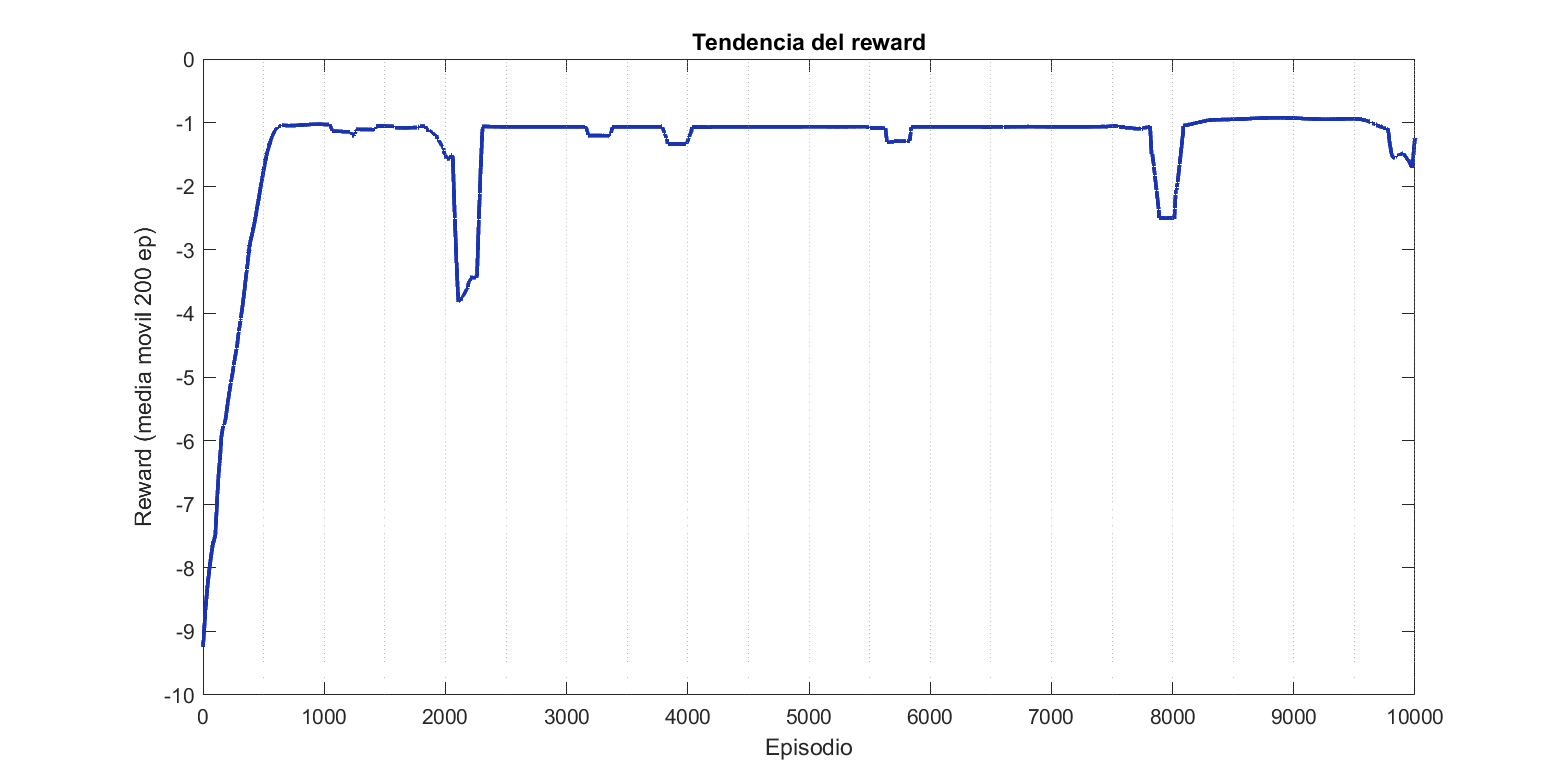
\includegraphics[width=0.85\textwidth]{02_reward_moving_average}
  \caption{Media móvil de 200 episodios del reward. Se aprecia una meseta larga
  ($\approx$episodio 600 a 10\,000) con dos colapsos súbitos ($\approx$2100 y
  $\approx$7800) que luego se recuperan --- firma clásica de inestabilidad, no de
  convergencia suave.}
  \label{fig:reward}
\end{figure}

\begin{figure}[H]
  \centering
  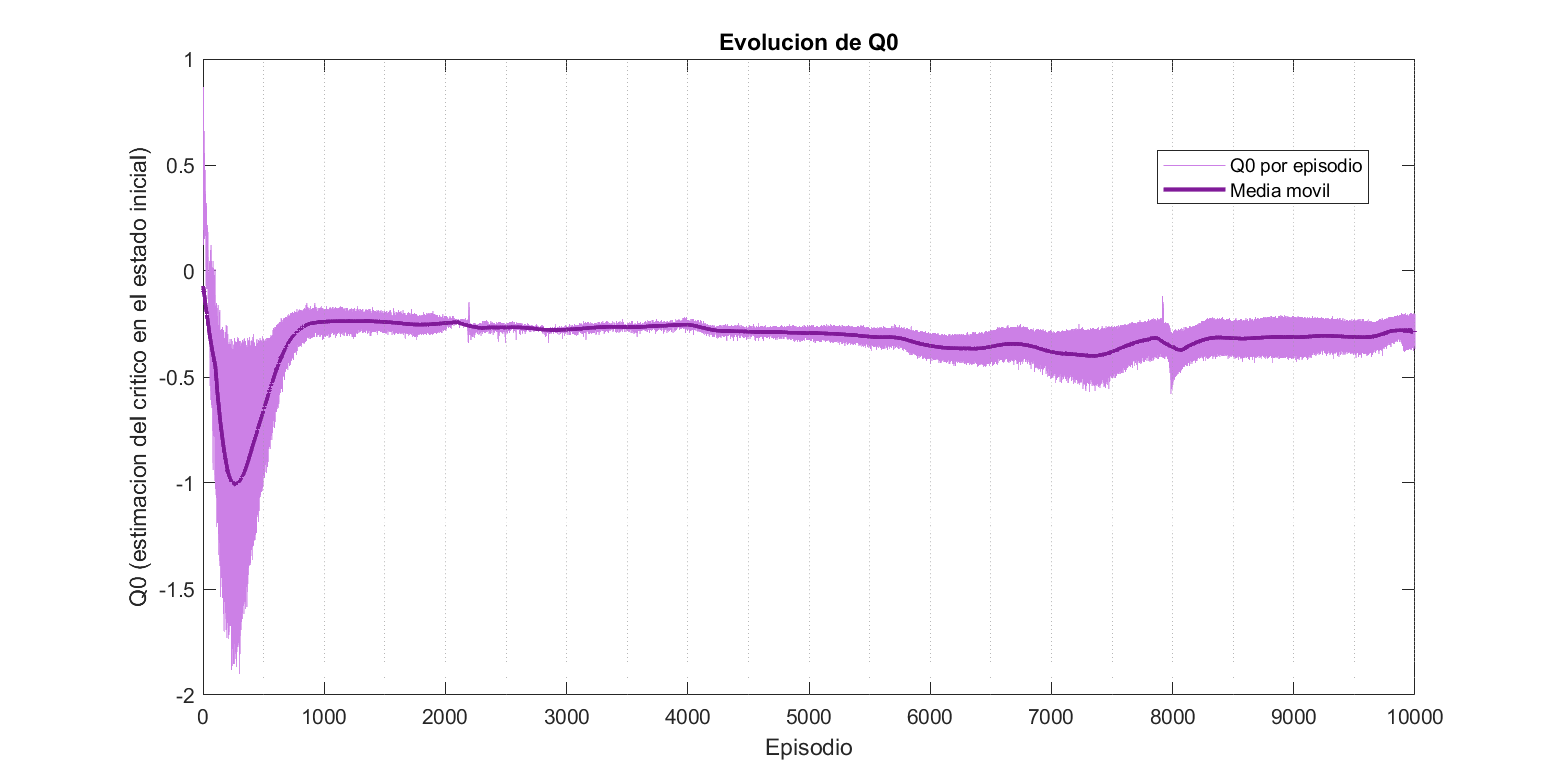
\includegraphics[width=0.85\textwidth]{03_episodeQ0_vs_episode}
  \caption{$Q_0$ (estimación del crítico en el estado inicial) por episodio. El
  \emph{drift} no monótono --- se vuelve más negativo durante la meseta de reward,
  luego se recupera --- indica que el crítico tiene dificultad para valorar de forma
  estable una política que apenas cambia de comportamiento.}
  \label{fig:q0}
\end{figure}

\subsection{Saturación del actor: el hallazgo central}

\begin{figure}[H]
  \centering
  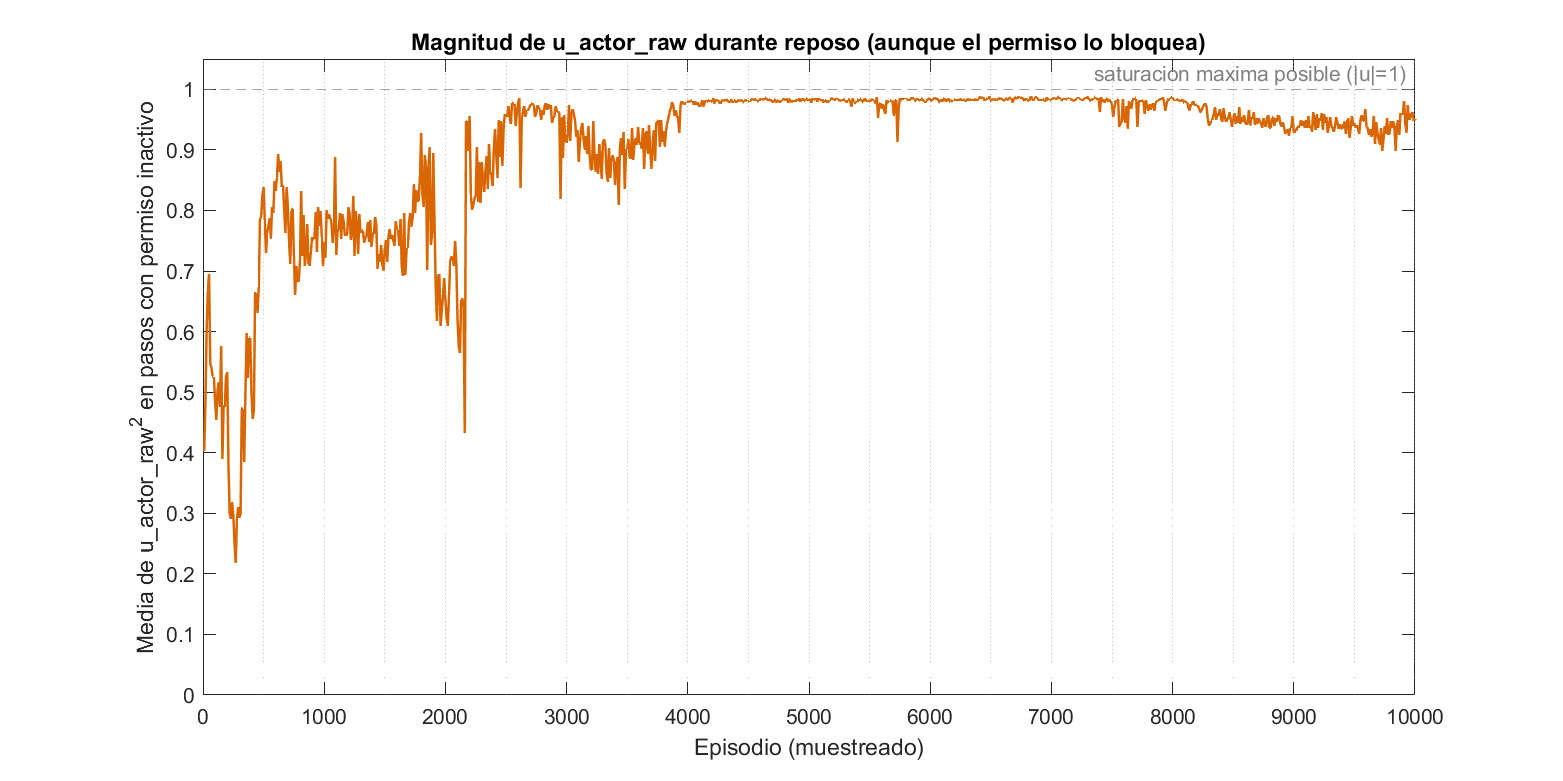
\includegraphics[width=0.85\textwidth]{10_restRawActionL2_vs_episode}
  \caption{Media de $u_{actor,raw}^2$ durante pasos con \texttt{motionPermission}
  inactivo (reposo), muestreada cada 10 episodios de entrenamiento. Sube de
  $\approx$0.5 a casi 1.0 (saturación máxima posible) hacia el episodio 4000, y se
  mantiene ahí. El gate bloquea correctamente esta salida --- pero el actor mismo
  nunca deja de intentar producir una acción extrema, incluso en reposo.}
  \label{fig:restraw}
\end{figure}

Verificación cuantitativa directa sobre acciones activas (evaluación determinista, sin
ruido): en los checkpoints Agent4000 y Agent6000, \textbf{el 100\% de las acciones
crudas activas tienen $|u_{raw}|\geq0.95$} --- el actor colapsó a un controlador tipo
relé (\emph{bang-bang}), no a control proporcional aprendido.

\begin{figure}[H]
  \centering
  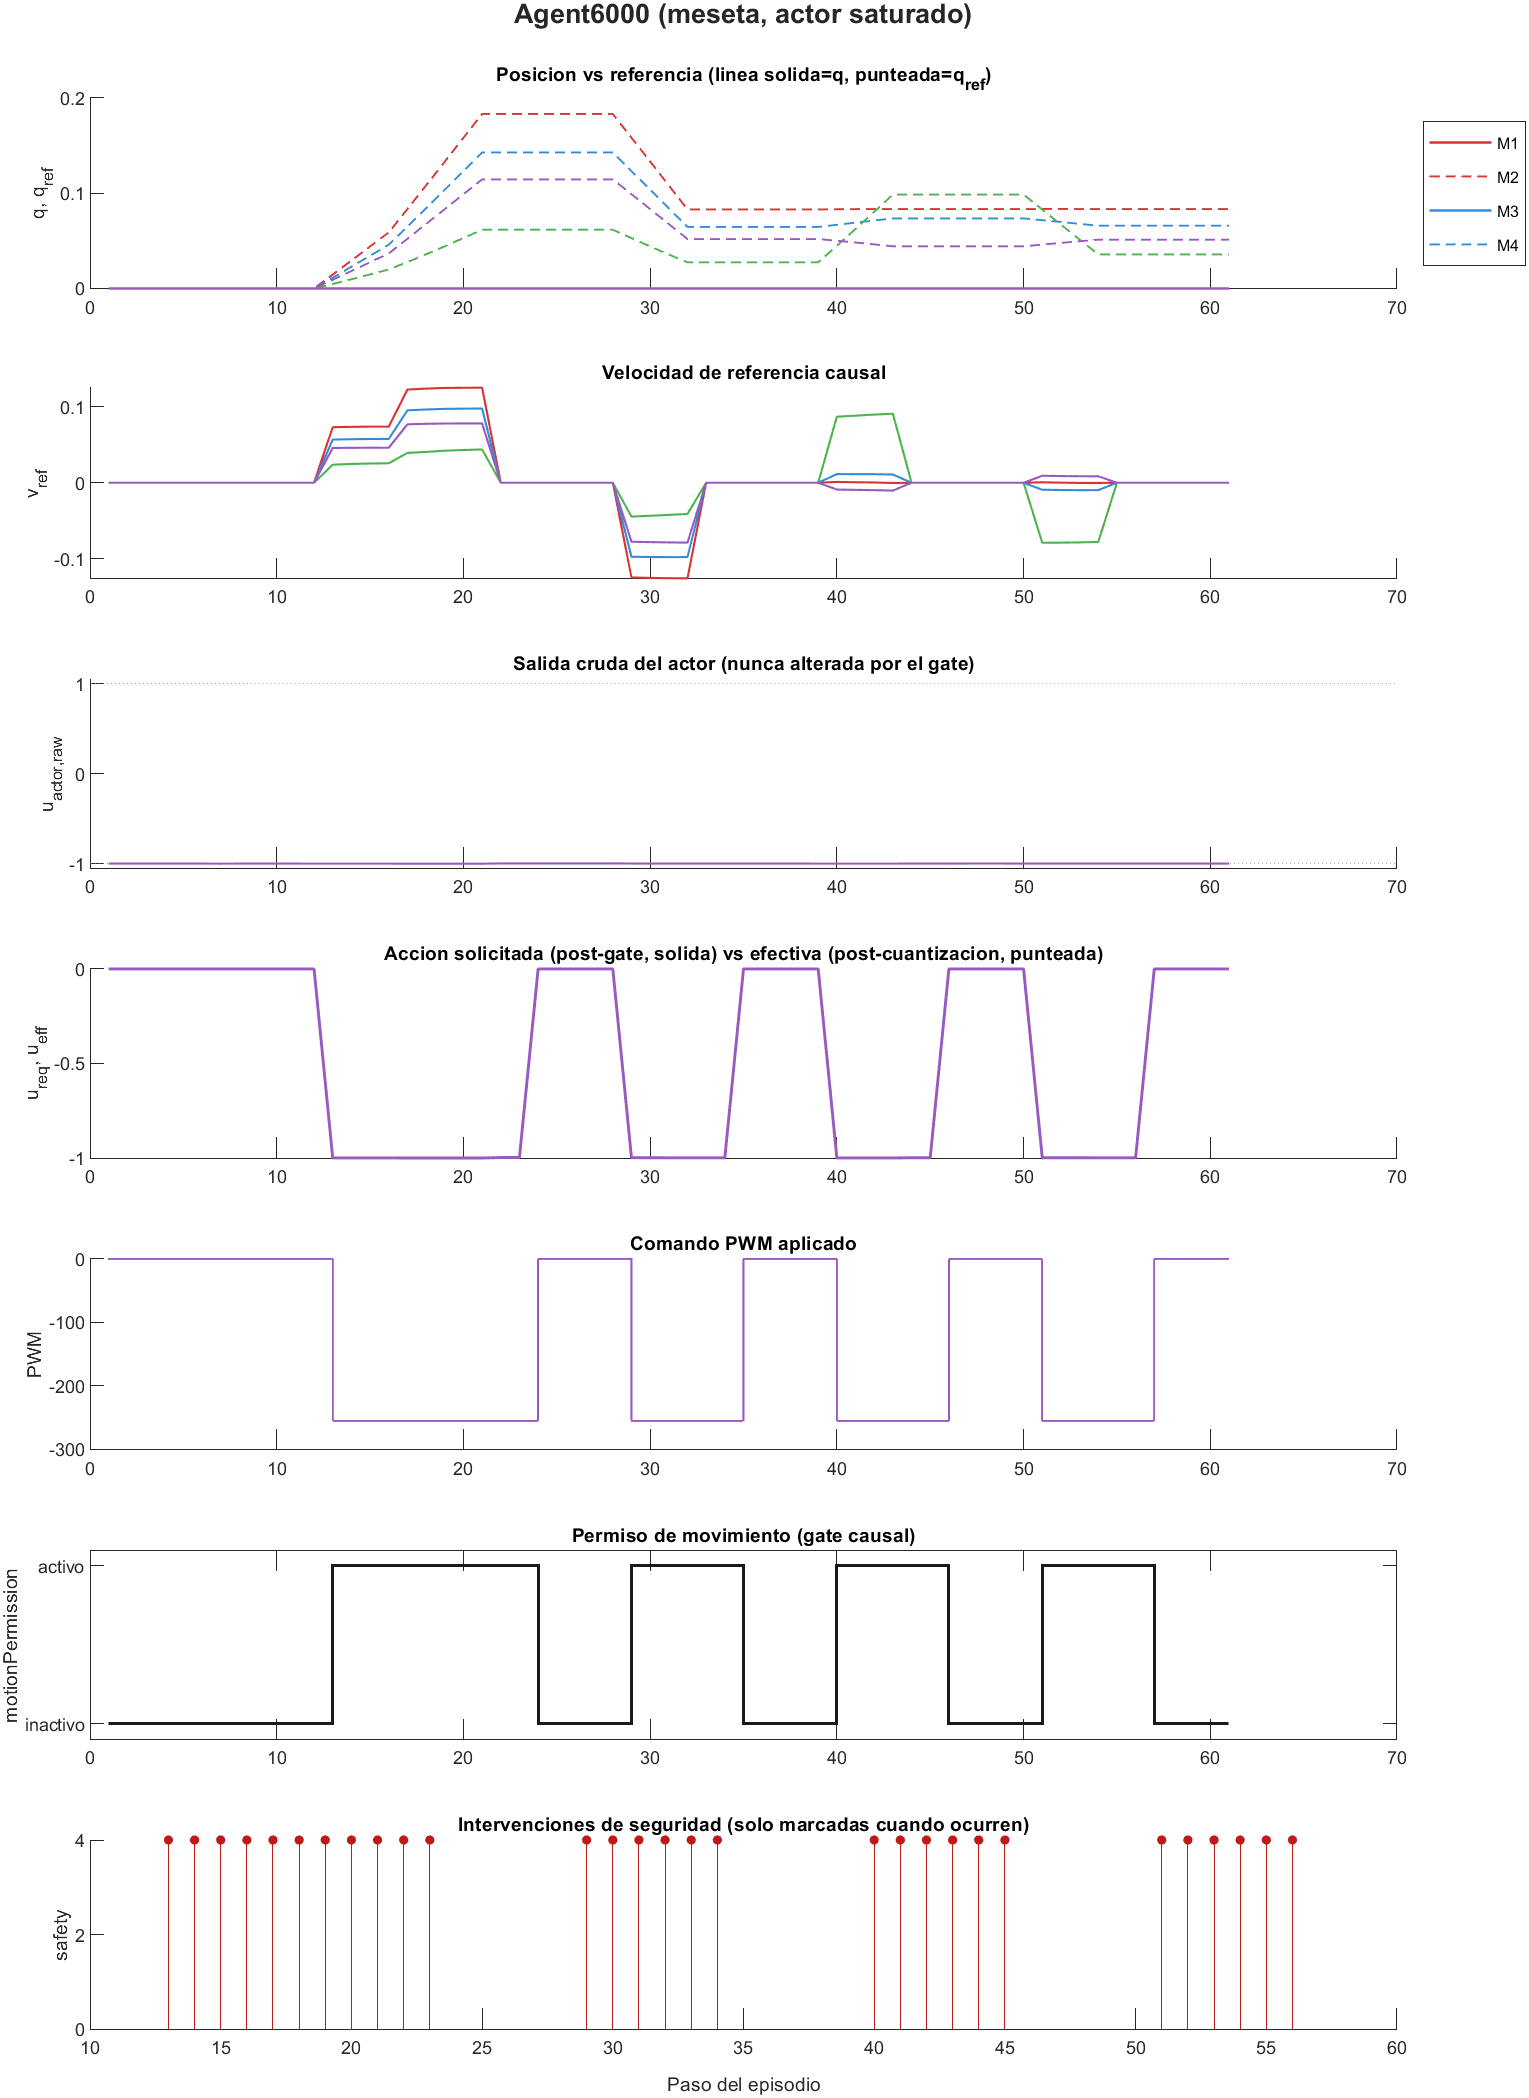
\includegraphics[width=\textwidth]{agent6000_episode1}
  \caption{Episodio de evaluación de Agent6000. Panel de $u_{actor,raw}$: la salida
  cruda del actor se mantiene en una banda estrecha cercana a $-0.8$/$-0.9$
  virtualmente todo el episodio, sin importar la fase de reposo o actividad ---
  evidencia visual directa de la saturación.}
  \label{fig:agent6000}
\end{figure}

\begin{figure}[H]
  \centering
  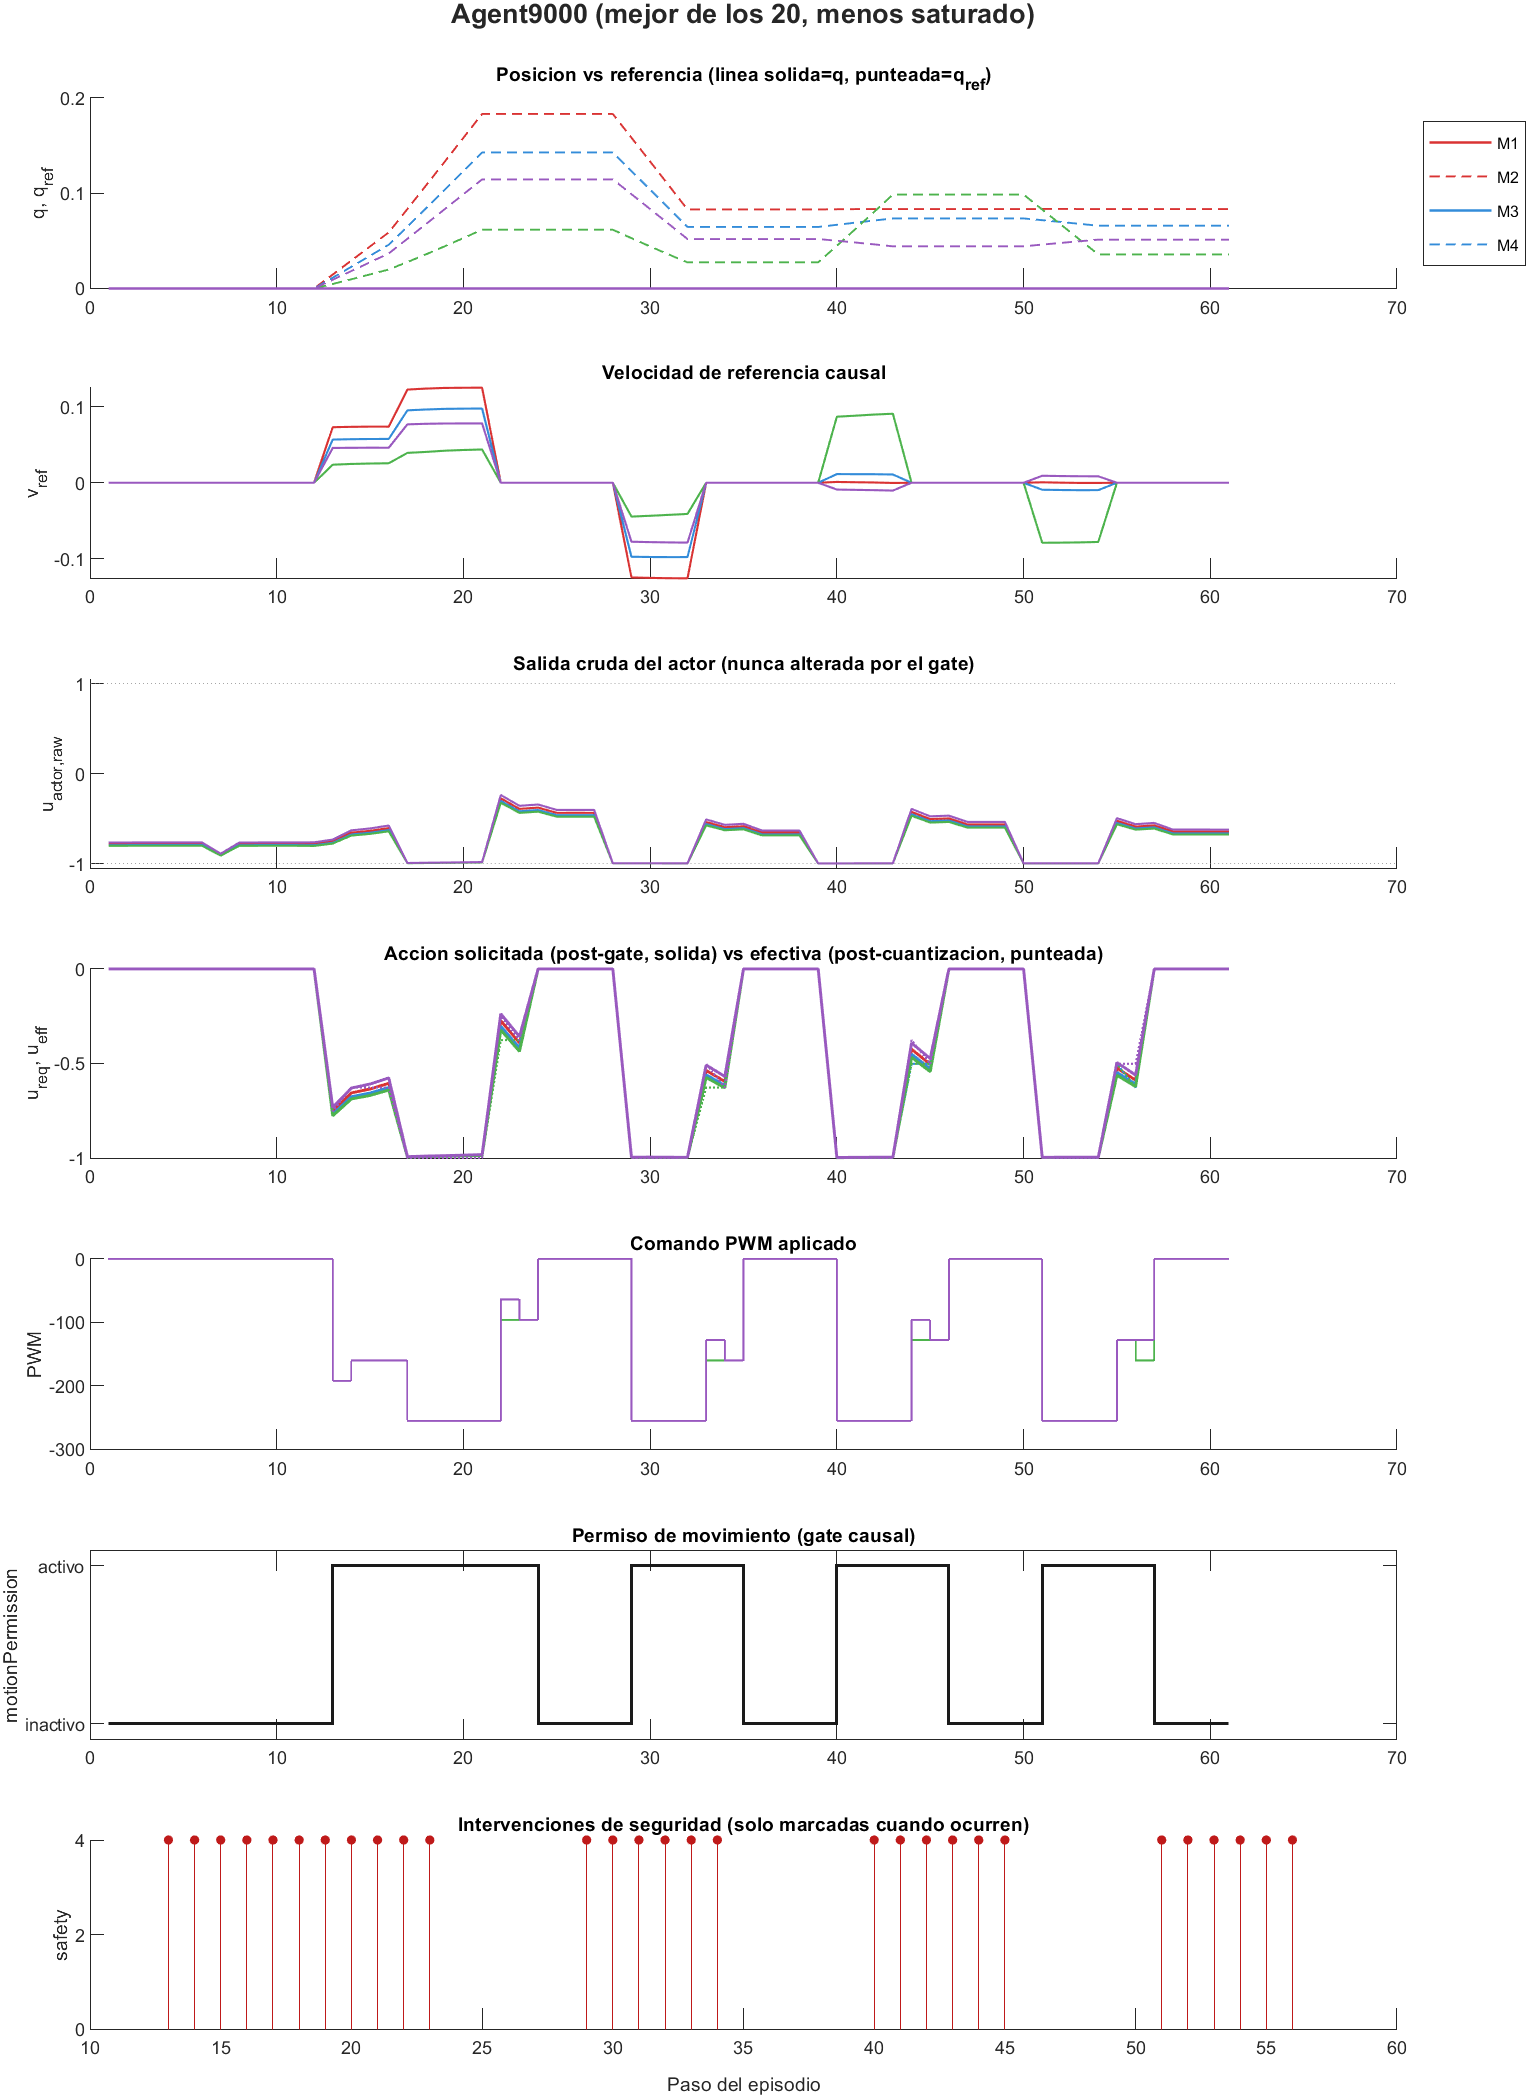
\includegraphics[width=\textwidth]{agent9000_episode1}
  \caption{Episodio de evaluación de Agent9000, el checkpoint menos saturado de los
  20. El seguimiento $q$ vs $q_{ref}$ es visualmente muy ajustado; el PWM y la acción
  efectiva caen exactamente a cero en cada ventana de reposo (\texttt{motionPermission}
  inactivo).}
  \label{fig:agent9000}
\end{figure}

\subsection{Resultados de todos los checkpoints}

\begin{table}[H]
\centering\small
\begin{tabular}{rrrrrrr}
\toprule
Checkpoint & trackingMse & actionL2 raw & actionL2 ef. & satFrac & restPWM$\neq$0 & safety \\
\midrule
Agent200+gate (baseline) & 0.0097 & --- & 0.1220 & --- & 0 & --- \\
\midrule
500 & 0.01374 & 0.811 & 0.434 & 0.367 & 0 & 3200 \\
1000 & 0.00609 & 0.857 & 0.457 & 0.415 & 0 & 2900 \\
2000 & 0.00954 & 0.838 & 0.419 & 0.383 & 0 & 2900 \\
4000 & 0.00609 & 0.990 & 0.475 & 0.475 & 0 & 2900 \\
6000 & 0.00609 & 0.996 & 0.475 & 0.475 & 0 & 2900 \\
8000 & 0.00609 & 0.993 & 0.475 & 0.475 & 0 & 2900 \\
8500 & 0.00616 & 0.774 & 0.367 & 0.244 & 0 & 2900 \\
9000 & 0.00619 & 0.718 & \textbf{0.340} & \textbf{0.238} & 0 & 2900 \\
9500 & 0.00655 & 0.742 & 0.344 & 0.238 & 0 & 2900 \\
10000 & 0.00688 & 0.811 & 0.351 & 0.246 & 0 & 2900 \\
\bottomrule
\end{tabular}
\caption{Subconjunto representativo del \texttt{checkpoint\_comparison.csv} completo
(20 filas). \texttt{restPWMNonZeroFraction}=0 en los 20 checkpoints, sin excepción.}
\label{tab:checkpoints}
\end{table}

\textbf{Mejor checkpoint:} \textbf{Agent9000} --- el de menor \texttt{actionL2}
efectivo y menor fracción de saturación entre los 20, con \texttt{trackingMse} todavía
mejor que el baseline. Ningún checkpoint iguala o supera de forma convincente a
Agent200+\texttt{motionPermission} en \emph{ambas} dimensiones (tracking \emph{y}
esfuerzo/seguridad) simultáneamente: los mejores en tracking (1000--8000) tienen
esfuerzo 3--4$\times$ mayor y casi el doble de intervenciones de seguridad que el
baseline; los de menor esfuerzo (8500--10000) siguen muy por encima del baseline en
\texttt{actionL2} y muestran tracking ligeramente peor que su propio óptimo intermedio.

\subsection{Clasificación}

\begin{quote}
\textbf{LONG\_TRAINING\_RESULT = UNSTABLE}
\end{quote}

Razones combinadas (no solo reward, según lo exigido): (1) meseta de reward de
$\approx$7500 episodios con dos colapsos súbitos y recuperación; (2) \emph{drift} no
monótono de $Q_0$; (3) saturación casi total del actor (100\% de acciones activas con
$|u_{raw}|\geq0.95$ en varios checkpoints intermedios); (4) \texttt{actionL2} 3--4$\times$
el baseline en todos los checkpoints; (5) intervenciones de seguridad casi el doble del
baseline. La única dimensión perfecta en las 20 evaluaciones es
\texttt{restPWMNonZeroFraction=0} --- el gate externo cumplió su función incluso frente
a un actor patológicamente saturado, validando la robustez arquitectónica de
\texttt{motionPermission} como capa \emph{separada} del entrenamiento del actor.

\subsection{Causa raíz y corrección propuesta}

La tasa de decaimiento de exploración (\texttt{explorationStdDecayRate=1e-4}) se
heredó sin cambios del perfil de ETAPA 6, calibrado para el horizonte de Agent200
(200 episodios $\times$ 61 pasos $\approx$12\,200 pasos totales, terminando con un
multiplicador de exploración $\approx$0.295$\times$, nunca llega al piso). Sobre
10\,000 episodios ($\approx$610\,000 pasos), esa misma tasa hace que la desviación de
exploración llegue a su piso (\texttt{explorationStdMin=0.02}) dentro del primer 1--2\%
del entrenamiento, dejando $\approx$98\% de la campaña con exploración casi nula. Junto
a una capa de salida \texttt{tanh} acotada, esto es una trampa de saturación conocida
en RL continuo: una vez que las preactivaciones crecen lo suficiente, el gradiente a
través de \texttt{tanh} se anula, y sin ruido de exploración sostenido no hay mecanismo
efectivo de escape.

\textbf{Corrección de un solo factor:} escalar \texttt{explorationStdDecayRate}
proporcionalmente al horizonte de entrenamiento, de forma que la exploración termine
en el mismo multiplicador relativo que experimentó Agent200
(\texttt{computeNoGloveStage7uExplorationDecayRate.m}, con 4 pruebas deterministas).
Nada más se modifica: actor, decoder, estado, reward, dataset, planta, seguridad,
cuantización y gate permanecen exactamente iguales.

\subsection{Validación corta}

Se validó con una campaña corta antes de considerar otra campaña de 10\,000 episodios,
por instrucción explícita. Corrida:
\texttt{stage7u\_exploration\_fix\_validation}, 1000 episodios,
\texttt{explorationStdDecayRate} calculada automáticamente
($\approx2\times10^{-5}$, ver \texttt{run\_metadata.mat} de esa corrida), comparada
contra el checkpoint Agent1000 de la campaña original (misma cantidad de episodios,
misma semilla, tasa de decaimiento original $10^{-4}$):

\begin{table}[H]
\centering\small
\begin{tabular}{lrrrr}
\toprule
Agent1000 & fracAbs$\geq$0.95 (activo) & mediaCuad. (activo) & mediaCuad. (reposo) & trackingMse \\
\midrule
Original ($10^{-4}$) & 0.8534 & 0.9508 & 0.7722 & 0.00609 \\
Con corrección ($\approx2\times10^{-5}$) & \textbf{0.7824} & \textbf{0.8874} & \textbf{0.6051} & 0.00610 \\
\bottomrule
\end{tabular}
\caption{Comparación directa al mismo número de episodios (1000). La corrección
reduce la saturación en las cuatro métricas de forma consistente (8.3 puntos
porcentuales menos de acciones activas saturadas, 21.6\% menos energía cuadrática de
$u_{actor,raw}$ en reposo) sin perjudicar el \texttt{trackingMse}, que permanece
esencialmente idéntico.}
\label{tab:validacion-corta}
\end{table}

La mejora es real, consistente y en la dirección esperada, aunque todavía modesta a
1000 episodios --- exactamente lo esperable, dado que el beneficio de mantener
exploración activa por más tiempo se acumula sobre un horizonte mucho más largo
(el efecto completo sólo puede confirmarse repitiendo la campaña de 10\,000 episodios
con la corrección). Esto satisface el criterio de "mejora antes de autorizar otra
campaña larga" fijado como precondición.

\section{Arquitectura de software}

\subsection{\texttt{Env.m}}
Clase principal (\texttt{classdef Env < rl.env.MATLABEnvironment}). Propiedades
inmutables fijadas una sola vez en el constructor desde \texttt{configurables()}
(entre ellas \texttt{motionPermissionEnabled}, ETAPA 7U); propiedades mutables llevan
todos los \emph{logs} por episodio (\texttt{actionLog}, \texttt{actionWarpLog},
\texttt{actionSatLog}, \texttt{actionPwmLog}, \texttt{motionPermissionLog},
\texttt{rewardInfoLog}, \ldots).

\subsection{\texttt{reset.m}}
Establece el estado inicial: para la línea \texttt{emgIntent}, fija
$q_{ref}=q$, $v_{ref}=0$, acción efectiva previa $=0$ \emph{directamente}, sin invocar
el decodificador --- el primer estado del episodio nunca depende de una ventana EMG
"falsa". Los episodios de tipo \emph{Closing} (relajados) parten del conteo de encoder
crudo \texttt{[0,0,0,0]} (exactamente \texttt{positionMin} normalizado); los de tipo
\emph{Opening} fuerzan \texttt{closeHand()} seguido de un \texttt{toc(10000)} --- que,
como se documentó en \S\ref{sec:etapa7t}, converge al equilibrio de la curva empírica
del simulador, no necesariamente a \texttt{positionMax=1}.

\begin{lstlisting}
% pseudocodigo simplificado de reset() para referenceSource=="emgIntent"
initialEncoderNorm = encoderNormCalculator(motorData);
intentTarget   = initialEncoderNorm;     % q_ref = q
intentVelocity = zeros(4,1);             % v_ref = 0
prevEffectiveActionForState = zeros(4,1);
State = calculateState(emg, motorData);  % NO se llama al decoder aqui
\end{lstlisting}

\subsection{\texttt{step.m}}
Orquesta, en orden estrictamente causal: cuantización de interfaz $\to$
\textbf{gate \texttt{motionPermission} (ETAPA 7U, antes de \texttt{remapActionForActuator})}
$\to$ cuantización PWM $\to$ envío a la planta $\to$ lectura de hardware/simulador
$\to$ cómputo de reward (con la acción \emph{efectiva}) $\to$ \emph{sólo después},
avance del decodificador de intención con la EMG recién leída (\texttt{advanceIntentReference})
$\to$ construcción del estado $t+1$.

\begin{lstlisting}
rawAction = action;
warpedAction = warp(rawAction);               % interfaz de accion
motionPermission = this.intentGateState.isActive;   % ETAPA 7U
if this.motionPermissionEnabled
    warpedAction = double(motionPermission) * warpedAction;
end
[effectiveAction, appliedPwm] = remapActionForActuator(warpedAction);
% ... enviar a planta, leer, calcular reward(effectiveAction) ...
% SOLO DESPUES:
advanceIntentReference(emg_nueva, currentEncoderNorm);  % actualiza q_ref/v_ref/gate
State_next = calculateState(...);
\end{lstlisting}

\subsection{\texttt{calculateState.m} / \texttt{buildObservationLayout.m}}
\texttt{calculateState} arma el vector de estado según \texttt{observationVariant},
delegando el contrato de índices (auditable) a \texttt{buildObservationLayout}, que
define exactamente los rangos de cada bloque (Sección de \texttt{intentMarkov60}).

\subsection{\texttt{advanceIntentReference.m} / decoder}
Invoca \texttt{mapEmgToIntentVelocity} (decoder + gate de histéresis) y
\texttt{updateIntentReference} (integración acotada), y --- sólo para la variante de
62 dimensiones --- \texttt{updateIntentDeclaredRestHoldState}. Devuelve además un
registro de procedencia (\texttt{intentProvenanceLog}) con \texttt{gateActive} por
transición, reutilizado extensamente en las auditorías offline de ETAPA 7T/7U.

\subsection{Reward: \texttt{trackingIntentActionRateReward.m}}
Función pura respecto de \texttt{Env}: recibe la acción efectiva y un contexto
explícito (incluida la acción previa) --- ningún estado oculto de la clase se lee
directamente, lo que la hace trivialmente testeable.

\subsection{Seguridad: \texttt{limitSimulationPosition.m}}
Adaptador externo al simulador puro; con \texttt{enabled=false} es una identidad
exacta. Nunca se modifica por \texttt{motionPermission} --- son capas ortogonales.

\subsection{\texttt{prosthesis\_simulator.m}}
Simulador basado en curvas empíricas grabadas por motor/velocidad/dirección
(\S\ref{sec:etapa7t}), no en un modelo físico paramétrico.

\subsection{\texttt{saveEpisode.m}}
Persiste todos los \emph{logs} de \texttt{Env} a un \texttt{.mat} por episodio,
incluyendo (desde ETAPA 7U) \texttt{motionPermissionLog} y
\texttt{motionPermissionEnabled}.

\subsection{\texttt{configurables.m}}
Único punto de verdad de la configuración; soporta \emph{overrides} vía
\texttt{setConfigurablesOverride}/\texttt{clearConfigurablesOverride} para experimentos
reproducibles sin tocar los valores por defecto. Valida invariantes cruzados (p.~ej.
\texttt{motionPermissionEnabled} exige \texttt{referenceSource="emgIntent"}).

\subsection{Workflows de \emph{training}/\emph{test} y scripts ETAPA 7U}
\begin{itemize}
  \item \texttt{run\_no\_glove\_stage7u\_motion\_permission\_ablation.m}: contrafactual
    offline exacto (sin recargar el actor).
  \item \texttt{run\_no\_glove\_stage7u\_closed\_loop\_confirmation.m}: confirmación en
    lazo cerrado real con Agent200 recargado.
  \item \texttt{run\_no\_glove\_stage7u\_optional\_long\_training.m}: entrena
    (\texttt{motionPermissionEnabled=true} desde el episodio 1), guarda checkpoints
    periódicos, y evalúa \textbf{todos} sobre el mismo conjunto de test determinista ---
    nunca asume que el último es el mejor.
  \item \texttt{computeNoGloveStage7uExplorationDecayRate.m}: la corrección de un solo
    factor de la Sección~\ref{sec:campana-10k}.
  \item \texttt{buildNoGloveStage7uTrainingFigures.m} /
    \texttt{plotNoGloveStage7uEpisode.m}: reconstrucción de figuras de entrenamiento y
    test sin reentrenar.
\end{itemize}

\section{Siguiente fase: Myo real, sin prótesis física}
\label{sec:myo}

Por instrucción explícita, esta fase se prepara \textbf{sólo si} la arquitectura y los
resultados finales son suficientemente válidos. Dado que la campaña de 10\,000 episodios
se clasificó \texttt{UNSTABLE} (Sección~\ref{sec:campana-10k}), \textbf{esa precondición
no se cumple todavía}: este informe reporta únicamente la auditoría del código Myo
histórico ya existente, sin construir el pipeline de captura en vivo.

\textbf{Hallazgos principales de la auditoría} (código, no documentación):
\begin{itemize}
  \item \texttt{Myo.m} delega la conexión real al SDK vendorizado \emph{MyoMex}
    (Thalmic Labs, discontinuado $\approx$2018); no hay binario MEX compilado en el
    repositorio, y el SDK probablemente no está disponible en este entorno.
  \item \texttt{Env.m} bloquea explícitamente Myo real combinado con la línea
    \texttt{emgIntent} (\texttt{Env:EmgIntentRequiresPrerecorded}); hoy no existe una
    ruta de código para "solo captura Myo" sin arrastrar el guante real/\texttt{FakeGlove}.
  \item \texttt{simMotors=true} \textbf{no} bloquea por sí solo una conexión Myo real
    (confirmado también en \texttt{00\_baseline\_audit.md}); no existe ningún flag
    formal de \emph{shadow/dry-run} en el código.
  \item \texttt{Myo.readEmg()} descarta los \emph{timestamps} reales por muestra; no
    hay detección de desconexión, reconexión ni paquetes perdidos durante la sesión.
  \item \texttt{FakeMyo} genera EMG en rango $[0,1)$; el Myo real entrega $[-1,1]$ ---
    cualquier prueba con \texttt{FakeMyo} no es representativa de la escala real.
  \item Una prueba histórica de compuerta de reposo con Myo real ya falló
    (\texttt{Failed\_InconsistentGate}, 0/2 corridas aceptadas).
\end{itemize}

Estos hallazgos quedan documentados como insumo directo para cuando la precondición se
cumpla; no se implementa código de captura Myo en este informe.

\section{Conclusiones}

\begin{enumerate}
  \item La arquitectura \texttt{motionPermission} está validada de forma robusta,
    offline y en lazo cerrado real, con el actor congelado de Agent200: mejora
    \texttt{trackingMse} en 21\% y reduce \texttt{actionL2} en 50.6\%, con supresión
    perfecta de PWM de reposo.
  \item Entrenar un actor nuevo \emph{con} el gate activo desde el episodio~1, durante
    10\,000 episodios, es arquitectónicamente sano en el sentido más importante
    ---\texttt{motionPermission} nunca dejó pasar PWM no solicitado, en ninguno de los
    20 checkpoints--- pero el propio entrenamiento TD3 fue inestable: el actor colapsó
    a un controlador saturado tipo relé durante la mayor parte de la campaña.
  \item Se identificó una causa raíz concreta y verificable (tasa de decaimiento de
    exploración mal escalada al horizonte de 10\,000 episodios) y se implementó una
    corrección de un solo factor, sin tocar ningún otro componente de la arquitectura.
  \item Ningún checkpoint de la campaña de 10\,000 episodios supera de forma
    convincente a Agent200+\texttt{motionPermission}; el mejor (Agent9000) se acerca en
    tracking pero sigue muy por encima en esfuerzo y seguridad.
  \item La siguiente fase (Myo real) queda auditada pero no iniciada, a la espera de
    que una campaña corregida confirme aprendizaje estable.
\end{enumerate}

\end{document}
